\subsection{Tipos de sistemas de enclavamiento}

    Los primeros sistemas de enclavamiento implementados fueron mecánicos \cite{Paper_179}. Estos utilizaban palancas, como las que se visualizan en la Figura \ref{fig:enclavamiento_1}, para comandar los cambios de vías y semáforos. Una palanca que habilite una ruta se encuentra bloqueada mecánicamente (enclavada) hasta que todas las palancas que afecten a los elementos ferroviarios correspondientes a esa ruta se encuentre en la posición que garanticen que la ruta es segura. De la misma manera, una vez habilitada una ruta, no es posible mecánicamente mover una palanca que habilite una ruta contraria y, por lo tanto, lleve a dos formaciones a colisionar frontal o lateralmente.
    
        \begin{figure}[H]
            \centering
            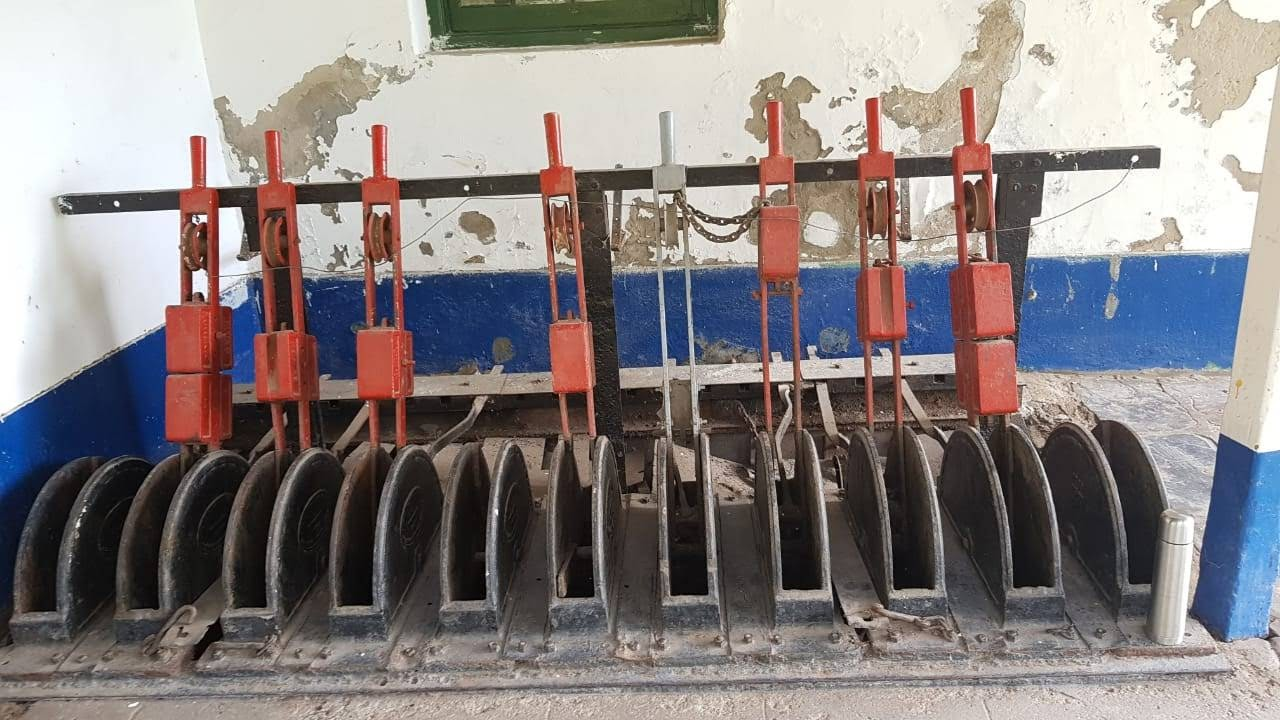
\includegraphics[width=1\textwidth]{Figuras/palancas.jpg}
            \centering\caption{Sistema de enclavamiento mecánico basado en palancas.}
            \label{fig:enclavamiento_1}
        \end{figure}

    Aunque hoy en día las tecnologías mas modernas ya no utilizan bloqueos mecánicos, se sigue utilizando el término \textit{enclavamiento}. En lugar de palancas y mecanismos de bloqueo, se utilizan circuitos lógicos, tanto eléctricos como electrónicos, y lógica programable que permitan garantizar el mismo objetivo: verificar condiciones previo a autorizar una ruta y prohibir la habilitación de rutas conflictivas con las actualmente activas.

    A comienzos del siglo XX se empezaron a utilizar sistemas de enclavamiento electromecánicos en entornos urbanos y semi-urbanos. Hoy en día este sistema es de los mas utilizado en muchos países \cite{Paper_179}, sobretodo en áreas rurales donde los sistemas tardan mas en actualizarse en comparación con las áreas urbanas. Un sistema de enclavamiento electromecánico se basa en relés (Figura \ref{fig:enclavamiento_2}) y circuitos de vía. Los circuitos eléctricos implementados con relés determinan la lógica del enclavamiento y son necesarios unas pocas decenas de relés para operar una derivación ferroviaria, pero cientos a miles para una estación terminal de gran tamaño \cite{Paper_199}.

    \begin{figure}[H]
        \centering
        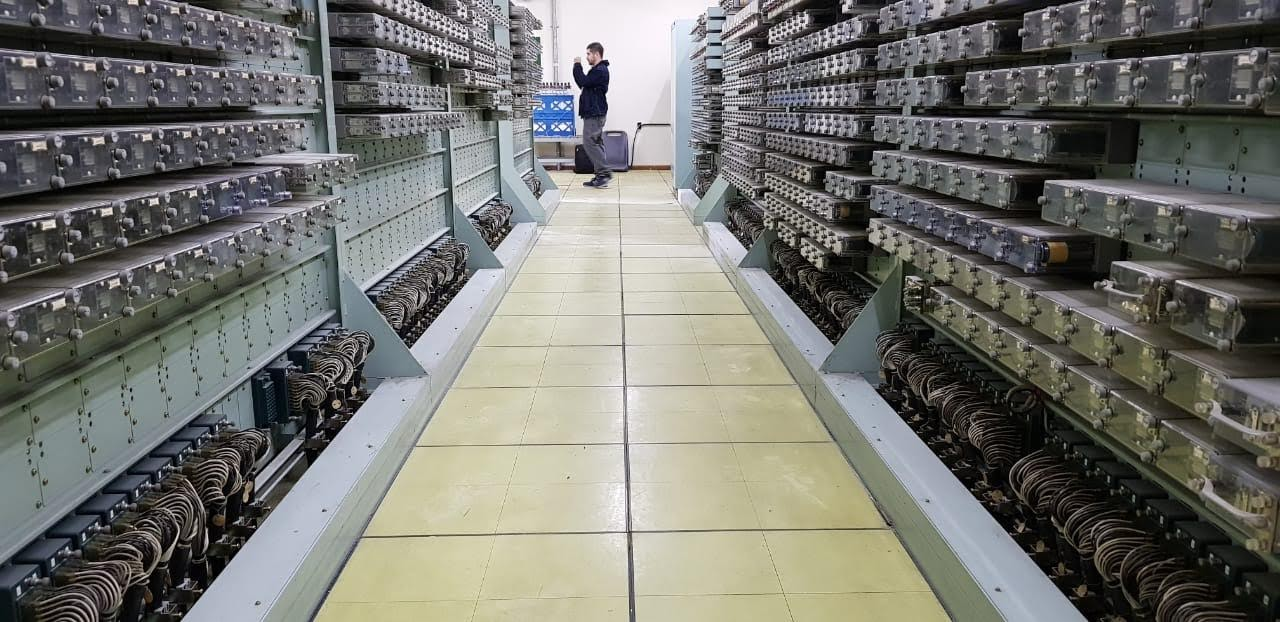
\includegraphics[width=1\textwidth]{Figuras/relees.jpg}
        \centering\caption{Sistema de enclavamiento electromecánico basado en relés.}
        \label{fig:enclavamiento_2}
    \end{figure} 
    
    Los sistemas de enclavamiento electromecánicos son comandados por un operario mediante un panel de control (Figura \ref{fig:enclavamiento_3}). El operario solicita al sistema de enclavamiento las rutas que el conductor ferroviario necesita para transitar por la vía. El sistema de enclavamiento solamente habilitará las rutas seguras, indicando al conductor que puede avanzar mediante un semáforo de aspecto verde o amarillo. En caso de que la ruta no sea habilitada, el sistema \textit{enclavará} los estados de los elementos ferroviarios pertenecientes a esa ruta y le indicará al conductor que no puede continuar su recorrido con un semáforo de aspecto rojo. El operario puede volver a pedir la ruta si las condiciones del sistema cambiaron.
    
    \begin{figure}[H]
        \centering
        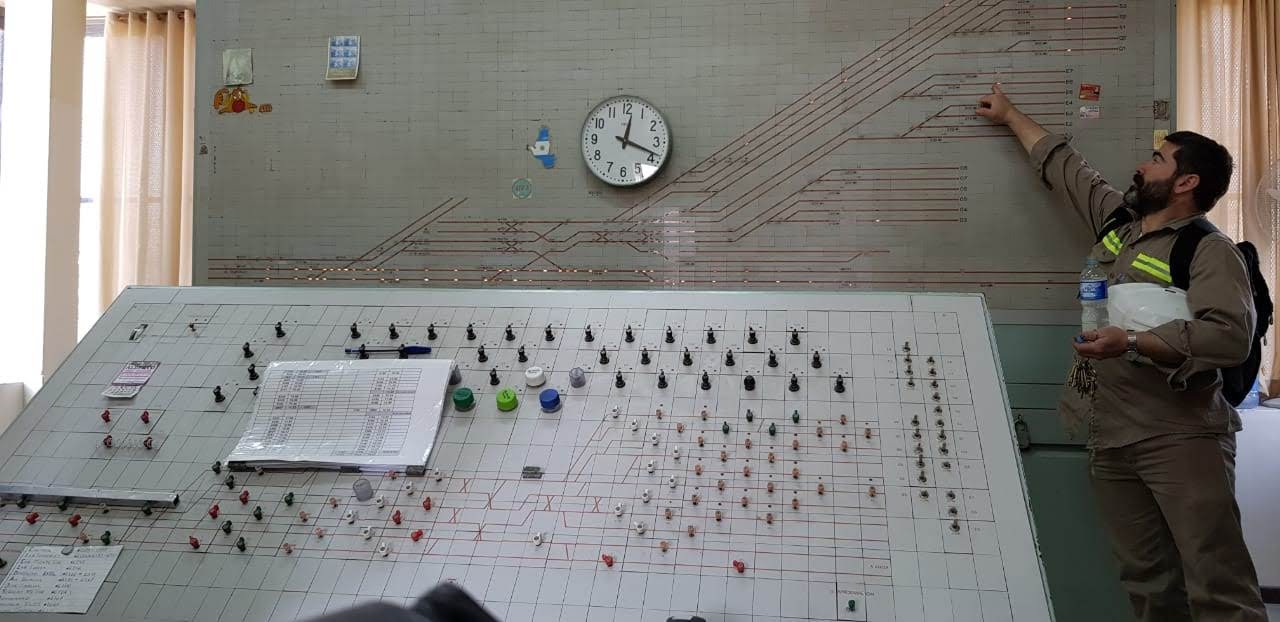
\includegraphics[width=1\textwidth]{Figuras/llavallol.jpg}
        \centering\caption{Panel de control central de un sistema de enclavamientos.} %TODO QUITAR A ELADIO
        \label{fig:enclavamiento_3}
    \end{figure}

    En la actualidad, los sistemas de enclavamiento mas modernos son electrónicos, basados en microprocesadores, PLCs (Controlador Lógico Programable, del inglés Programmable Logic Controllers), o FPGAs (Matriz de puerta programable en campo, del inglés Field-programmable Gate Array) \cite{Paper_8,Paper_22,Paper_24,Paper_25,Paper_28,Paper_31,Paper_34,Paper_35,Paper_36}. Estas tecnologías presentan la ventaja de ser reprogramables una vez instaladas, lo que aporta flexibilidad al diseño, escalabilidad y robustez \cite{Paper_38,Paper_46,Paper_47,Paper_118,Paper_124,Paper_128,Paper_130,Paper_131,Paper_133,Paper_135,Paper_204}. Además, ocupan mucho menos espacio que su contraparte electromecánica, reduciendo los costes de infraestructura, consumo eléctrico y mantenimiento. Se utilizan principalmente en redes de procesamiento distribuido, debido a su integración de forma nativa con protocolos de comunicación industrial diseñados para entornos ferroviarios \cite{Paper_125,Paper_37,Paper_41}. Adicionalmente, los sistemas electrónicos pueden ser fácilmente auditados y redundados, para aumentar su fiabilidad y comprobar su nivel de seguridad \cite{Paper_23,Paper_29,Paper_43,Paper_49,Paper_97,Paper_98,Paper_132,Paper_140}.